\ifdefined\XeTeXversion\RequirePackage[T1]{fontenc}\fi
\documentclass[conference]{IEEEtran}
\usepackage[T1]{fontenc}
\usepackage{balance}
\usepackage{cite,amsmath,amssymb,graphicx,booktabs,array,tabularx}
\usepackage{tikz}
\usetikzlibrary{arrows.meta,positioning,fit}
\usepackage{listings,xcolor}
\usepackage[hyphens]{url}
\usepackage[hidelinks]{hyperref}
\urlstyle{same}
\newcolumntype{Y}{>{\raggedright\arraybackslash}X}

% Restrained visual hierarchy; IEEEtran controls the page geometry and headings.
\definecolor{ReportInk}{HTML}{24465E}
\definecolor{ReportMuted}{HTML}{526270}
\definecolor{ReportRule}{HTML}{9AAAB5}
\definecolor{ReportTint}{HTML}{F2F5F7}
\definecolor{CodeString}{HTML}{486650}
\newenvironment{keypoints}{\begin{itemize}\setlength{\itemsep}{2pt}%
\setlength{\parsep}{0pt}}{\end{itemize}}
\renewcommand{\arraystretch}{1.12}
\setlength{\tabcolsep}{4pt}
\newcommand{\BIBdecl}{\raggedright}
\lstdefinelanguage{CSharp}{keywords={new,return,public,private,static,void,null},
 sensitive=true,morecomment=[l]{//},morestring=[b]"}
\lstdefinelanguage{Dart}{keywords={return,null,final,Future,void,async,await},
 sensitive=true,morecomment=[l]{//},morestring=[b]'}
\lstset{basicstyle=\ttfamily\scriptsize,breaklines=true,columns=fullflexible,
 numbers=left,numberstyle=\tiny\color{ReportMuted},numbersep=6pt,
 keywordstyle=\color{ReportInk}\bfseries,stringstyle=\color{CodeString},
 commentstyle=\color{ReportMuted}\itshape,backgroundcolor=\color{ReportTint},
 frame=single,rulecolor=\color{ReportRule},framerule=0.35pt,
 xleftmargin=12pt,xrightmargin=2pt,framexleftmargin=3pt,
 aboveskip=8pt,belowskip=8pt,captionpos=b,showstringspaces=false,
 keepspaces=true,tabsize=2}
\tikzset{box/.style={draw=ReportInk,fill=ReportTint,rounded corners=1pt,
 align=center,font=\scriptsize,minimum height=7mm,inner sep=2pt,text width=22mm},
 arr/.style={-{Latex[length=1.5mm]},draw=ReportInk,thin}}

\newcommand{\code}[1]{\texttt{#1}}
\hyphenation{PostgreSQL RabbitMQ PayOS Flutter}
\begin{document}
\title{CosmoQ Cinema: Web Ticket Booking and Cinema\\Management with Flutter and ASP.NET Core}
\author{
\IEEEauthorblockN{\small Nguyen Nguyen Ngu (QE190064), Dao Thi Thanh Huong (QE190046), Pham Ngo Bich Tram (QE1900100)\\
\small Nguyen Hoang Ngoc Chau (QE190088), Nguyen Xuan Dang Khoa (QE1900126)}
\IEEEauthorblockA{Student Developers, Class: SEK19B.Net\\
Department of Software Engineering\\
FPT University Quy Nhon Campus, Binh Dinh, Vietnam}
\IEEEauthorblockA{\textbf{Huynh Vang} --- Project Advisor, Lecturer\\
Department of Software Engineering, FPT University Quy Nhon Campus\\
Binh Dinh, Vietnam \quad\textbar\quad vangh@fe.edu.vn}}
\maketitle
\begin{abstract}
Cinema ticketing requires customer purchases and cinema operations to agree on
showtimes, seat ownership, and payment state. CosmoQ Cinema implements these
interactions through Flutter Web customer and administration entry points and
a shared ASP.NET Core 8 backend. This report reconstructs the implementation
from source, dependency manifests, SQL schemas, tests, and deployment scripts.
A YARP gateway routes JSON requests to authentication, movie, and booking
services. Entity Framework Core with Npgsql accesses six PostgreSQL databases;
transactional reservation rows and a seat/showtime uniqueness constraint support
seat contention handling. The browser layer uses named routes, explicit session
state, remote repositories, responsive layouts, and token-refresh coordination.
PayOS checkout and reconciliation, RabbitMQ outboxes, notification records,
counter sales, promotions, and loyalty functions are analyzed within their
verified boundaries. Seventeen isolated booking-service unit tests and
twenty-one gateway tests passed; backend compilation succeeded, with four
nullable warnings in MovieService. Container-dependent verification was blocked
by an unavailable Docker daemon. The Flutter suite passed 209 tests; both browser entry points compiled,
and analysis retained one informational lint. These checks remain separate
from source implementation, and no live payment or production
deployment is claimed. The contribution is a traceable account of the Web
system's coordination mechanisms and remaining verification obligations.
\end{abstract}
\begin{IEEEkeywords}
Cinema booking, Flutter Web, ASP.NET Core, PostgreSQL, JWT, PayOS, RabbitMQ, cinema management.
\end{IEEEkeywords}

\section{Introduction}
Cinema ticketing couples a customer-facing purchase with operational tasks such
as maintaining schedules, allocating seats, collecting payments, and admitting
customers. A booking interface must therefore coordinate information that can
change between browsing a show and completing checkout. A seat visible as free
is not necessarily still available when a customer submits an order. Likewise,
a browser returning from a payment page is not sufficient evidence that the
cinema has received money. These are the concrete coordination problems
addressed by the inspected CosmoQ implementation, rather than measured claims
about the shortcomings of a particular cinema's previous process.

CosmoQ Cinema implements customer booking and cinema-management workflows
through Flutter browser applications and an ASP.NET Core backend. This paper
examines the Web system: the customer application built from \code{main.dart}
and the administration application built from \code{main\_admin.dart}. They are
distinct entry points in one Flutter source project, not independently verified
frontend repositories. A mobile build shares customer code and backend APIs,
but its platform behavior is outside the primary scope of this paper.
Repository evidence, including source-level dependencies and SQL, establishes
the implementation described here \cite{client,webui,deployment,db}.

The principal engineering contributions are the following integrated mechanisms:
\begin{keypoints}
\item \textbf{Browser workflow composition.} Named navigation, session recovery,
responsive customer pages, and role-aware management entry points share remote API adapters.
\item \textbf{Server-controlled reservation.} Backend pricing, transactional seat
holds, and a seat/showtime uniqueness constraint coordinate competing purchases.
\item \textbf{Payment and operational follow-up.} Provider reconciliation and
outbox events connect booking state to notifications, refunds, and cinema operations.
\end{keypoints}
Concessions, promotions, loyalty balances, reviews, check-in, and notification
records support these workflows. Their source implementation does not establish
a production deployment, successful live payment, or performance improvement
over another ticketing system.

\subsection{Evidence and Scope}
Inspection used repository revision \code{55642353331f} and database submodule
revision \code{e455d297c76b}, retrieved on October 28, 2026. Manifests,
entry points, controllers, services, repositories, entity mappings, SQL,
platform configuration, tests, and CI definitions were cross-checked. Existing
requirements documents served as navigation aids rather than proof that a
feature works. Official framework references explain the technologies, while
repository references substantiate CosmoQ-specific behavior.

The analysis distinguishes implemented source, mocked test dependencies,
configured external integrations, and behavior not executed during this review.
In particular, a test using a fake PayOS client cannot validate a merchant
account, banking settlement, or public webhook delivery. Section VII reports
the checks actually executed and their limits.

\section{System Architecture Overview}
\subsection{Deployment Units and Communication}
Figure~\ref{fig:architecture} summarizes the verified Web topology. Browser
requests use JSON over HTTP through a YARP gateway. AuthService manages identity;
MovieService contains movie and showtime/room functionality; BookingService
contains booking, payment, notification, and related business services. Each is
an ASP.NET Core executable. Their separate Compose service definitions and
inter-service HTTP/event communication support describing the backend as a
service-based deployment. This does not imply independently scalable production
infrastructure or a separate service for every business module
\cite{gateway,movie,booking,deployment}.

\begin{figure*}[t]
\centering
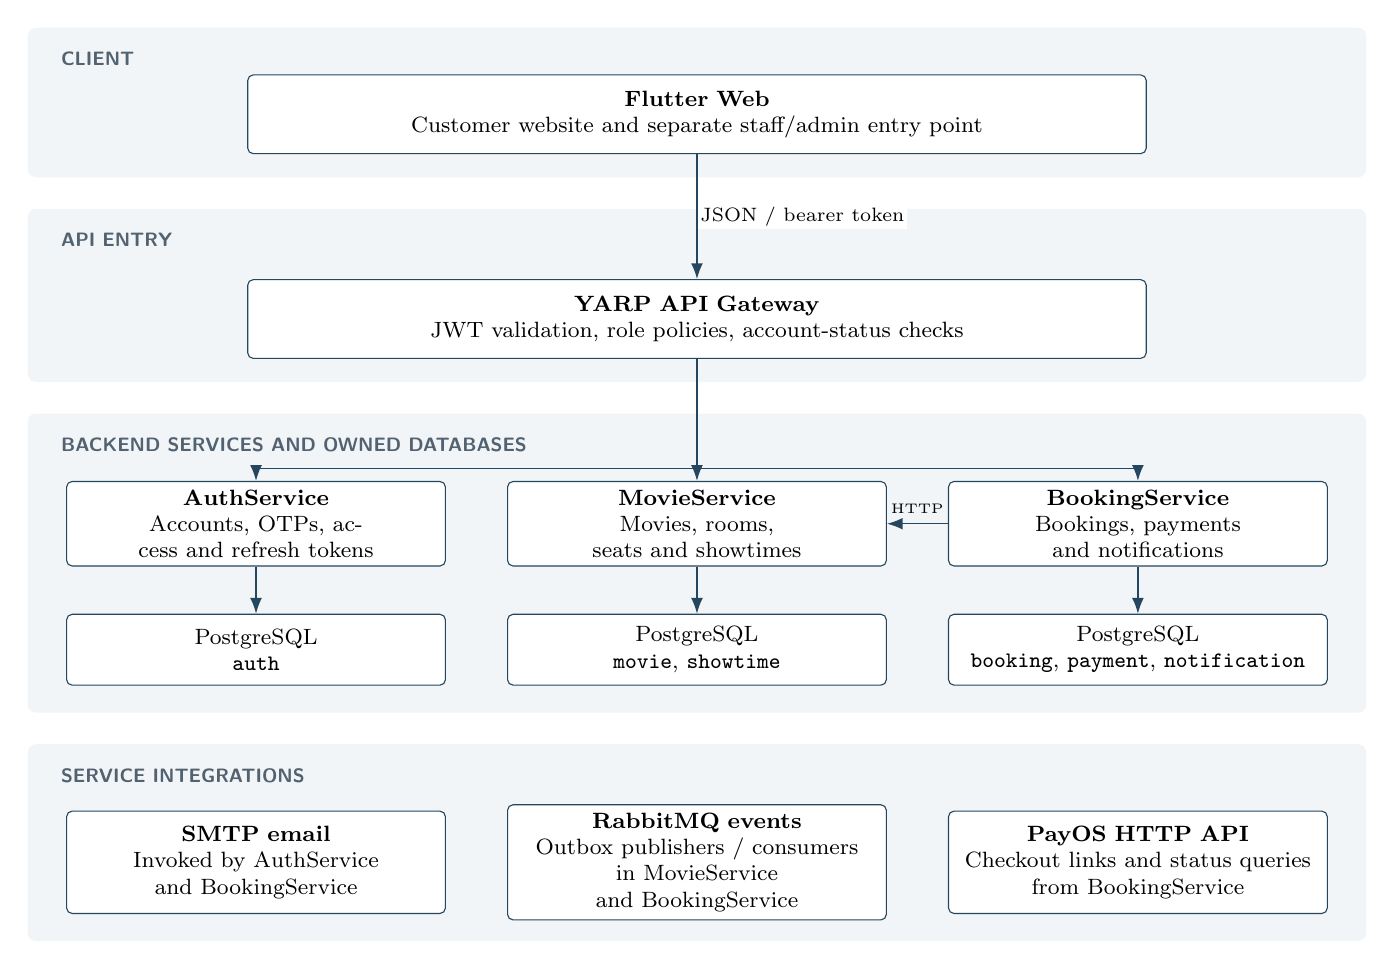
\begin{tikzpicture}[x=1mm,y=1mm,
 layer/.style={font=\sffamily\scriptsize\bfseries,text=ReportMuted,anchor=west},
 component/.style={draw=ReportInk,rounded corners=2pt,fill=white,
 align=center,font=\footnotesize,inner sep=3pt},
 connection/.style={-{Latex[length=2mm]},draw=ReportInk,line width=0.55pt}]
% Each horizontal band has a single purpose; external bindings never run through a database.
\fill[ReportTint,rounded corners=3pt] (0,8) rectangle (170,-11);
\fill[ReportTint,rounded corners=3pt] (0,-15) rectangle (170,-37);
\fill[ReportTint,rounded corners=3pt] (0,-41) rectangle (170,-79);
\fill[ReportTint,rounded corners=3pt] (0,-83) rectangle (170,-108);
\node[layer] at (3,4) {CLIENT};
\node[component,text width=112mm,minimum height=10mm] (client) at (85,-3)
 {\textbf{Flutter Web}\\Customer website and separate staff/admin entry point};
\node[layer] at (3,-19) {API ENTRY};
\node[component,text width=112mm,minimum height=10mm] (gateway) at (85,-29)
 {\textbf{YARP API Gateway}\\JWT validation, role policies, account-status checks};
\node[layer] at (3,-45) {BACKEND SERVICES AND OWNED DATABASES};
\node[component,text width=46mm,minimum height=10mm] (auth) at (29,-55)
 {\textbf{AuthService}\\Accounts, OTPs, access and refresh tokens};
\node[component,text width=46mm,minimum height=10mm] (movie) at (85,-55)
 {\textbf{MovieService}\\Movies, rooms, seats and showtimes};
\node[component,text width=46mm,minimum height=10mm] (booking) at (141,-55)
 {\textbf{BookingService}\\Bookings, payments and notifications};
\node[component,text width=46mm,minimum height=9mm] (authdb) at (29,-71)
 {PostgreSQL\\\code{auth}};
\node[component,text width=46mm,minimum height=9mm] (moviedb) at (85,-71)
 {PostgreSQL\\\code{movie}, \code{showtime}};
\node[component,text width=46mm,minimum height=9mm] (bookingdb) at (141,-71)
 {PostgreSQL\\\code{booking}, \code{payment}, \code{notification}};
\draw[connection] (client)--node[right,font=\scriptsize,fill=white,inner sep=1pt]
 {JSON / bearer token}(gateway);
\draw[connection] (gateway.south)--(85,-48)-|(auth.north);
\draw[connection] (gateway.south)--(movie.north);
\draw[connection] (gateway.south)--(85,-48)-|(booking.north);
\draw[connection] (booking.west)--node[above,font=\tiny]{HTTP}(movie.east);
\draw[connection] (auth)--(authdb);
\draw[connection] (movie)--(moviedb);
\draw[connection] (booking)--(bookingdb);
\node[layer] at (3,-87) {SERVICE INTEGRATIONS};
\node[component,text width=46mm,minimum height=13mm] at (29,-98)
 {\textbf{SMTP email}\\Invoked by AuthService\\and BookingService};
\node[component,text width=46mm,minimum height=13mm] at (85,-98)
 {\textbf{RabbitMQ events}\\Outbox publishers / consumers\\in MovieService and BookingService};
\node[component,text width=46mm,minimum height=13mm] at (141,-98)
 {\textbf{PayOS HTTP API}\\Checkout links and status queries\\from BookingService};
\end{tikzpicture}
\caption{Web system architecture with explicit service/database ownership and external integration bindings. Solid arrows show client/API and persistence paths.
The integration cards identify the backend services responsible for each external binding.
Database labels abbreviate the six \code{cinema\_\ldots\_db} names; all six use one PostgreSQL instance in Compose.}
\label{fig:architecture}
\end{figure*}


The gateway listens on host port 5000 in Compose. Backend and infrastructure
debug ports are generally bound to loopback, while the gateway is accessible
from the network. Route-to-cluster configuration selects the destination
service; downstream failures are translated into structured 503 or 504 responses.
BookingService calls MovieService for authoritative showtime and seat data,
forwarding the acting user's bearer token. RabbitMQ carries business events
after local transactions commit. Browser clients do not connect directly to
PostgreSQL or RabbitMQ \cite{gateway,booking,deployment}.

\subsection{Technology and Repository Organization}
Table~\ref{tab:stack} identifies technologies confirmed by dependencies and
active code. The installed verification SDK is Flutter 3.47.2 with Dart 3.13.2;
the Flutter CI workflow instead requests version 3.47.4. This is a reproducibility
distinction, not evidence that either version was used for a released website.
Backend projects target \code{net8.0}; the local build host uses .NET SDK 9.0.305.
\begin{table}[t]
\caption{Verified Web Technology Stack}\label{tab:stack}
\centering\footnotesize
\begin{tabularx}{\columnwidth}{@{}lYY@{}}\toprule
\textbf{Component} & \textbf{Technology} & \textbf{Responsibility}\\\midrule
Browser UI & Flutter, Dart, Material & Customer and administration views\\
Client API & Dart \code{http} & JSON requests and bearer tokens\\
Gateway & ASP.NET Core 8, YARP 2.3.0 & Routing and request policies\\
Backend & ASP.NET Core 8 & Controllers and business services\\
Persistence & EF Core 8, Npgsql; PostgreSQL 17 image & Mappings and SQL databases\\
Events & RabbitMQ.Client 7.2.1 & Outbox publication and consumers\\
Payment & PayOS HTTP integration & Checkout links and reconciliation\\
Operations & Docker Compose; OpenTelemetry & Local topology and telemetry\\\bottomrule
\end{tabularx}
\end{table}

The Flutter \code{lib} tree separates \code{app}, \code{admin}, \code{core},
\code{data}, and feature-oriented directories. \code{AppDependencies.remote}
constructs real service adapters, repositories, secure token storage, and a
token manager. Backend services register controller, business-service,
repository, and EF Core dependencies explicitly. Interface-backed repositories
are present, but a uniform Clean Architecture or domain-driven design is not
established by this organization. Flutter's architecture guidance provides
context for separation of UI and data access \cite{flutter}; CosmoQ's actual
dependency construction remains the relevant evidence \cite{client}.

\subsection{Persistence Boundaries}
Compose initializes six databases on one PostgreSQL instance. Their domain
suffixes are \code{auth}, \code{movie}, \code{showtime}, \code{booking},
\code{payment}, and \code{notification}; full names follow the
\code{cinema\_...\_db} convention.
MovieService owns two EF contexts and BookingService owns three. Thus six
database names do not imply six backend executables. Npgsql supplies the EF
Core provider \cite{npgsql}; source registration selects each database
\cite{auth,movie,booking,deployment}.

\section{Backend Design and Implementation}
\subsection{Identity and Access Services}
\textbf{Account lifecycle.} AuthService implements registration, email verification, login, refresh,
logout, profile changes, password changes, and administrative account operations.
Passwords and OTP values are hashed with BCrypt. JWT generation uses
HMAC-SHA256 and includes user identity and role claims. Refresh tokens are
generated from 64 cryptographically random bytes, stored in the authentication
database, and revoked when rotated. A logout revokes the supplied refresh token;
it is not described here as an instantaneous blacklist of every previously
issued access token \cite{auth}.

\textbf{Request authorization.} JWT validation checks issuer, audience, signature, and lifetime. Gateway policies
and downstream controller policies restrict privileged actions. Protected
gateway requests also query AuthService's current-account endpoint. Disabled
accounts are refused, and a mismatch between current roles and token roles
returns a role-change error. Failure to perform that check returns 503 rather
than forwarding an unchecked protected request \cite{gateway}. These are
concrete bearer-token mechanisms consistent with the ASP.NET Core model
\cite{jwt}, not a claim of OAuth/OpenID Connect federation.

\subsection{Catalog and Schedule Support}
MovieService provides movie browsing, detail retrieval, genres, title search,
and administrative editing. Its showtime code validates room membership of
requested seats, rejects shows that are not open or have started, and enforces
paired sweetbox selection when a partner exists. Seat prices derive from the
showtime price, presentation-format surcharge, and seat-type surcharge.
Room, seat, and schedule APIs support management screens rather than requiring
the browser to manipulate database records \cite{movie,webui}.

Showtime creation checks start/end ordering and room schedule conflicts through
the repository. Cancellation records a business event in the showtime database
outbox; BookingService consumes it to process affected bookings. These checks
show implemented business validation. They do not establish that all possible
concurrent administrative schedule edits have been tested in this environment.

\subsection{Booking Transactions and Seat Contention}
The booking controller derives the customer ID and email from authenticated
claims for self-service purchases. The service rejects duplicate seat IDs,
requests server-side seat prices, and calculates concessions from the active
menu. It loads showtime timing for later cancellation policy decisions. The
movie title normally comes from MovieService, although the code retains a
request-title fallback if no title is returned; therefore it would be inaccurate
to claim that every display field is exclusively server-derived \cite{booking}.

The transaction uses three complementary mechanisms \cite{booking,db,postgres}:
\begin{keypoints}
\item \textbf{Lock existing reservations.} PostgreSQL \code{FOR UPDATE} locks
the selected rows; booked seats and unexpired holds are rejected.
\item \textbf{Constrain new reservations.} The unique
\code{uq\_seat\_}\allowbreak\code{per\_showtime} key protects a seat/showtime pair before a row
exists to lock. A unique violation rolls back the transaction and returns a conflict.
\item \textbf{Commit related state.} The booking, seat snapshots, holds, and
outbox event are persisted in one local transaction.
\end{keypoints}
These are specific concurrency mechanisms; they do not establish an unrestricted
guarantee under every failure mode.

Listing~\ref{lst:seat} reproduces the relevant EF mapping. The database schema
contains the corresponding unique constraint. UI disabling alone would not
provide this protection; simultaneous browser sessions can submit the same
selection despite a recently refreshed map.
\begin{lstlisting}[language=CSharp,caption={Reservation uniqueness mapping from BookingDbContext.},label={lst:seat}]
entity.HasIndex(
    e => new { e.ShowtimeId, e.SeatId },
    "uq_seat_per_showtime")
  .IsUnique();
\end{lstlisting}

\subsection{Database Model and Relationships}
Figure~\ref{fig:data} shows a selected, verified relational subset. Solid edges
represent declared SQL foreign keys; dashed edges denote application-level ID
references across database boundaries. Authentication uses users, roles, a join
table, refresh tokens, and OTP records. Showtime storage relates rooms to seats
and showtimes. Booking storage keeps ticket-seat price snapshots and
concession lines. Payments relate to refunds within their own database
\cite{db,booking}.
\begin{figure}[t]
\centering
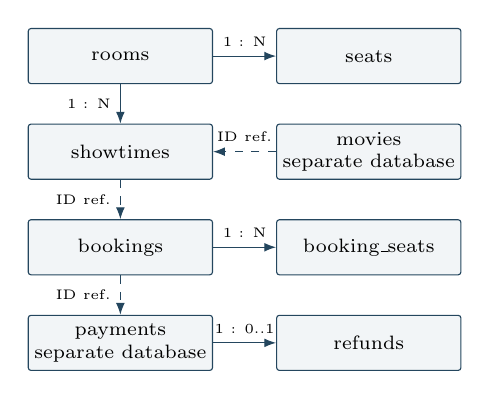
\begin{tikzpicture}[node distance=5mm and 8mm]
\node[box] (room) {rooms};
\node[box,right=of room] (seat) {seats};
\node[box,below=of room] (show) {showtimes};
\node[box,right=of show] (movie) {movies\\separate database};
\node[box,below=of show] (booking) {bookings};
\node[box,right=of booking] (bs) {booking\_seats};
\node[box,below=of booking] (payment) {payments\\separate database};
\node[box,right=of payment] (refund) {refunds};
\draw[arr] (room)--node[above,font=\tiny]{1 : N}(seat);
\draw[arr] (room)--node[left,font=\tiny]{1 : N}(show);
\draw[arr,dashed] (movie)--node[above,font=\tiny]{ID ref.}(show);
\draw[arr,dashed] (show)--node[left,font=\tiny]{ID ref.}(booking);
\draw[arr] (booking)--node[above,font=\tiny]{1 : N}(bs);
\draw[arr,dashed] (booking)--node[left,font=\tiny]{ID ref.}(payment);
\draw[arr] (payment)--node[above,font=\tiny]{1 : 0..1}(refund);
\end{tikzpicture}
\caption{Selected schema relationships reconstructed from SQL. Solid arrows
denote parent-to-child SQL foreign keys; dashed arrows denote logical ID
references. Reservations, identity, and other extension tables are omitted.}
\label{fig:data}
\end{figure}


Cross-database references such as a payment's booking ID are not PostgreSQL
foreign keys in the supplied schema. The reservation's booking ID is also not
declared as an SQL foreign key in the inspected base script. These distinctions
matter when discussing consistency: asynchronous handlers and application checks
coordinate business records, while database constraints cover only their
defined local scope. The figure is deliberately a partial ERD, not a claim to
reproduce every table or every entity-mapping detail.

Initialization SQL and incremental migrations are kept in the database
submodule. Compose mounts those files and runs an initialization script for
an empty volume, followed by a migration job. Additional SQL under the backend
tree updates movie metadata and reviews. The migration script excludes selected
demo-seeding migrations. This inspected path uses SQL scripts; no claim is made
that EF migration history governs the deployed schema \cite{deployment,db}.

\subsection{Payments and Event Delivery}
The PayOS adapter creates checkout links, queries orders, and cancels links.
It sends merchant headers and signs creation payloads with HMAC-SHA256.
Webhook handling validates the data signature before using fields, matches
the payment order and amount, and records the successful payment. A later
booking-confirmation conflict can initiate a refund request. These operations
are integrated in source; live merchant delivery was not exercised
\cite{booking,payos}.

\textbf{Asynchronous delivery.} Outbox publishers read unpublished events with \code{FOR UPDATE SKIP LOCKED},
publish persistent messages with publisher confirmations, and record publication
state. Consumers handle booking cancellation, payment/refund changes, email
notifications, and showtime cancellation. Event identifiers and uniqueness checks
support duplicate handling. This follows an at-least-once delivery approach:
a broker publish and database publication marker are not a single distributed
transaction. RabbitMQ confirms are useful evidence of broker acceptance, not
proof of exactly-once business effects or exactly-once email delivery
\cite{booking,rabbit}.

\section{Web Application Architecture and Implementation}
\subsection{Entry Points and Browser Navigation}
Both entry points restore a stored session before constructing their application.
The customer router maps named paths to movie, showtime, booking, payment,
notification, and account screens. Authentication-required routes redirect to
login while retaining a pending destination. Detail routes accept an identifier
and can reload their data when no in-memory navigation argument exists.
This is particularly relevant to browser refresh and shared links
\cite{client}.

The administration router classifies routes as public, staff, or admin. It
checks roles before creating protected pages. This improves navigation but is
not the security boundary: the backend independently authorizes management
operations. CI defines a customer Web build and a separate admin build using
\code{--base-href /admin/}. The configured build layout is evidence of packaging,
not proof that a hosting environment serves both correctly \cite{client,tests}.

\begin{table}[t]
\caption{Representative Browser Screens and Routes}\label{tab:routes}
\centering\footnotesize
\begin{tabularx}{\columnwidth}{@{}lYY@{}}\toprule
\textbf{View} & \textbf{Route or entry} & \textbf{Responsibility}\\\midrule
Customer home & \code{/home} & Browse and filter movies\\
Movie details & \code{/movies/\{id\}} & Metadata, reviews, showtimes\\
Seats & \code{/showtimes/}\allowbreak\code{\{id\}/seats} & Selection and availability\\
Booking detail & \code{/bookings/\{id\}} & Ticket and booking state\\
Payment & \code{/bookings/}\allowbreak\code{\{id\}/payment} & Checkout and reconciliation\\
Movie management & \code{/admin/movies} & Admin catalog editing\\
User management & \code{/admin/users} & Account and role operations\\
Staff workspace & \code{main\_admin.dart} & Counter sales and operations\\\bottomrule
\end{tabularx}
\end{table}

\subsection{State and API Abstractions}
\code{SessionState} extends \code{ChangeNotifier}; an
\code{InheritedNotifier} exposes authentication, the current user, and unread
notification count. Screens otherwise maintain local state for loading,
selection, filters, and errors. No evidence requires labeling this state system
as Bloc, Riverpod, or Redux. Repositories translate screen requests into
service calls; the shared API client handles JSON, timeouts, bearer headers,
and structured errors \cite{client}.

An authenticated 401 can trigger one refresh and a retry. Concurrent callers
share a pending refresh future to avoid independently rotating the same token.
Network failures retain the session where possible, whereas invalid refresh
credentials or account-status errors clear it. \code{SessionApp} then replaces
navigation with sign-in and displays the reason. These details connect the API
layer to visible browser behavior instead of relying on route guards alone.

\subsection{Responsive Presentation and Reuse}
The layout utility switches the main desktop arrangement at 900 logical pixels.
Wide customer pages use a top navigation frame; narrower layouts retain the
application-style bottom navigation. Shared width constraints distinguish forms,
reading views, and wide pages. \code{ResponsiveColumns} uses a separate local
constraint threshold, defaulting to 820 pixels, to stack a sidebar below content.
Consequently, there is not one universal breakpoint for every component
\cite{client,webui}.

Theme files define colors, spacing, radii, and typography; common components
provide buttons, panels, network-image fallbacks, loading, empty, and error
states. Web-specific trailer implementations and counter-ticket printing use
browser facilities through conditional imports. This is verified platform
branching, not evidence that all browsers or assistive technologies were
evaluated. Table~\ref{tab:modules} summarizes the main functional divisions.

\begin{table}[t]
\caption{Major Web Functional Modules}\label{tab:modules}
\centering\footnotesize
\begin{tabularx}{\columnwidth}{@{}lYY@{}}\toprule
\textbf{Module} & \textbf{Implemented responsibility} & \textbf{Principal layers}\\\midrule
Catalog & Browse, details, genres, trailers & Flutter; MovieService\\
Booking & Seats, summary, history, QR ticket & Flutter; BookingService\\
Checkout & PayOS link and status checks & Flutter; payment service\\
Counter & Walk-in booking and cash payment & Admin UI; booking/payment APIs\\
Management & Movies, rooms, schedules, users & Admin UI; authorized services\\
Retention & Promotions, points, reviews & Client views; booking database\\
Notifications & Lists, read state, email records & Flutter; event handlers\\\bottomrule
\end{tabularx}
\end{table}

\section{Core Business Workflows}
\subsection{Discovery to Reservation}
The home screen requests now-showing or coming-soon data, genre filters, and
title search. Search input is debounced by 350 milliseconds in source.
Movie details retrieve open showtimes; the catalog repository bounds customer
schedule selection to a seven-day window and can fetch subsequent pages while
that window is relevant. Room seats and occupied seat IDs are requested in
parallel and combined into a client map \cite{client,webui}.

\textbf{Selection versus reservation.} Selection is initially local. Every five seconds, the seat screen attempts to
refresh availability while it is current; seats no longer free are removed
from the local selection, including paired-seat adjustments. Submitting the
summary creates the backend hold described in Section III. A conflict still
requires the customer to choose again. The repository therefore implements
polling plus transactional reservation, rather than a SignalR or WebSocket
seat-lock channel \cite{client,booking}.

\subsection{Pricing and Checkout}
For ticket subtotal $S$, applicable promotion discount $D$, concession subtotal
$C$, and redeemed loyalty points $q$, the booking code computes
\begin{equation}
T = S-D+C-1000q .\label{eq:price}
\end{equation}
The loyalty helper restricts redemption to at most
$\lfloor 0.5(S-D+C)/1000\rfloor$ points, additionally bounded by the customer's
balance. Promotion calculation caps the discount at 90\% of ticket value and
rounds it down to a 1,000-VND increment. These are implementation constants,
not measured economic outcomes \cite{booking}.

Figure~\ref{fig:flow} summarizes checkout. The payment page opens the returned
PayOS URL and displays the booking's expiry. It polls booking state every five
seconds and invokes provider verification every sixth eligible poll. Browser
return parameters identify an order to verify; the backend remains responsible
for deciding payment success. A timer or a successful redirect alone does not
confirm the ticket \cite{client,booking}.
\begin{figure}[t]
\centering
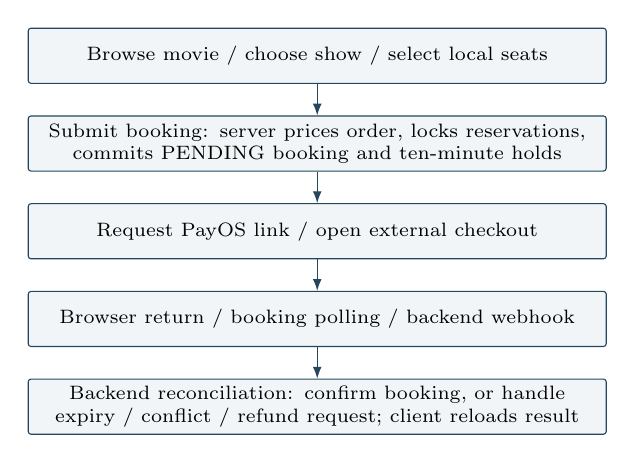
\begin{tikzpicture}[node distance=4mm]
\node[box,text width=72mm] (s) {Browse movie / choose show / select local seats};
\node[box,below=of s,text width=72mm] (b) {Submit booking: server prices order, locks reservations,\\commits PENDING booking and ten-minute holds};
\node[box,below=of b,text width=72mm] (p) {Request PayOS link / open external checkout};
\node[box,below=of p,text width=72mm] (v) {Browser return / booking polling / backend webhook};
\node[box,below=of v,text width=72mm] (r) {Backend reconciliation: confirm booking, or handle\\expiry / conflict / refund request; client reloads result};
\draw[arr] (s)--(b);\draw[arr] (b)--(p);\draw[arr] (p)--(v);\draw[arr] (v)--(r);
\end{tikzpicture}
\caption{Web reservation and checkout control flow. No client redirect or timer is itself proof of payment.}
\label{fig:flow}
\end{figure}


\subsection{Confirmation, Cancellation, and Operations}
Confirmed bookings expose history/detail views and QR ticket content. Customers
can request cancellation subject to server policy; the default paid-booking
cutoff is two hours before the show. A customer refund request sets
\code{REFUND\_PENDING} and retains seats until the refund decision. Staff
complete or reject refund processing through privileged APIs. The code records
manual transfer references; it does not implement an automatic banking refund
through a PayOS refund endpoint \cite{booking,webui}.

Staff workflows include counter booking, cash collection, booking lookup,
check-in, showtime operations, payment records, and notification handling.
Admin screens additionally manage movies, rooms, users, concessions,
promotions, and membership data. These are source-backed screen-to-service
paths, not a claim that every management path was manually exercised. Check-in
requires an eligible paid booking and a server-configured time window;
repeated admission is rejected by business logic \cite{booking,webui}.

\section{Security and Data Protection}
\subsection{Trust Boundaries}
The implementation places checks at three trust boundaries
\cite{auth,gateway,booking}:
\begin{keypoints}
\item \textbf{Identity and ownership.} Gateway/service authorization accompanies
UI routing. Booking reads check ownership; self-service creation uses identity claims.
\item \textbf{Order value.} Server pricing recalculates seat and concession
amounts instead of trusting totals submitted by the browser.
\item \textbf{Provider data.} Webhook signatures are checked before payment data
is used to confirm a booking.
\end{keypoints}
Password validation additionally accounts for BCrypt's input-length boundary.

\subsection{Browser Storage and Configuration}
The client actively uses \code{flutter\_secure\_storage} for access/refresh
tokens and user metadata. Writes are sequential, with a source comment
explaining first-write key creation on Web. Unreadable storage clears local
credentials. This establishes the chosen storage abstraction, not an
application-level guarantee against script execution or browser compromise.
The package documents HTTPS or localhost requirements for its Web backend
\cite{client,storage}.

\textbf{Deployment configuration.} Gateway CORS uses configured origins when present, but falls back to allowing
any origin if the list is empty. Fixed-window IP rate limits include a separate
authentication policy and return 429 responses. Compose passes secrets via
environment variables; the review did not open or publish credential values.
The supplied local topology exposes HTTP, so TLS termination is a deployment
requirement to verify, not an observed property of a live website. Seed
accounts and demonstration data should not be treated as a production identity
baseline \cite{gateway,deployment,db}.

\section{Testing, Verification, and Evaluation}
\subsection{Method and Observed Results}
Verification was performed on October 28, 2026. Table~\ref{tab:tests} separates
successful checks from environmental blocks and external operations that were
not attempted. No response-time, load, availability, coverage, or usability
metrics were collected. Build success demonstrates compilation, while unit and
widget results support only the exercised assertions \cite{tests,fluttertest}.
\begin{table}[t]
\caption{Verification Executed on October 28, 2026}\label{tab:tests}
\centering\footnotesize
\begin{tabularx}{\columnwidth}{@{}YY@{}}\toprule
\textbf{Check and method} & \textbf{Observed result / status}\\\midrule
BookingService isolated unit filter & \textbf{PASS}: 17 tests, zero failed\\
ApiGateway test project & \textbf{PASS}: 21 tests, zero failed\\
AuthService build & \textbf{PASS}: zero errors/warnings\\
MovieService build & \textbf{PASS}: zero errors; four nullable warnings\\
Flutter analysis & 1 informational lint; no errors/warnings\\
Flutter unit/widget suite & \textbf{PASS}: 209 tests after package restore\\
PostgreSQL/RabbitMQ integration suites & \textbf{BLOCKED}: Docker daemon unavailable\\
SQL/migration execution & \textbf{NOT EXECUTED}: no running database\\
Live PayOS, SMTP, deployed acceptance & \textbf{NOT EXECUTED}: external services not exercised\\
Customer/admin browser builds & \textbf{PASS}: both entry points compile\\\bottomrule
\end{tabularx}
\end{table}


After restoring the existing declared Flutter dependencies, the full
\code{flutter test --no-pub --reporter expanded} run passed 209 tests.
\code{flutter analyze --no-pub} reported one informational finding,
\code{curly\_braces\_in\_flow\_control\_structures}, in
\code{trailer\_url.dart:12}; no analysis errors or warnings remained.
The analyzer was therefore not a clean zero-finding run. The earlier
no-restore attempt failed because locally cached QR/sharing packages were
missing, and is not counted as a passed test run. No application source
was changed to obtain the restored-package result.

Both browser entry points also compiled successfully with
\code{flutter build web --no-pub --no-web-resources-cdn}; the admin build
selected \code{lib/main\_admin.dart} and base path \code{/admin/}.
These are compilation results, not browser-hosted acceptance tests.



The 17 isolated BookingService tests exercise signature handling and email
templates. The 21 gateway tests exercise request policy and failure behavior
with test infrastructure. Neither total should be interpreted as a live
deployment acceptance count. AuthService compiled without warnings; MovieService
compiled with four nullable-analysis warnings. BookingService and ApiGateway
compiled as part of their successful test runs.

\subsection{Test Doubles and Missing Runtime Evidence}
Booking integration fixtures use PostgreSQL Testcontainers and optionally a
real RabbitMQ container, but replace MovieService, PayOS, and SMTP with fake
clients. Flutter workflow tests likewise use fake repositories and plugin
substitutes. Their test names describe intended assertions, not evidence of
real merchant payments or actual email delivery \cite{tests}.

\textbf{Runtime verification boundary.} Docker's daemon was unavailable during this review, preventing the
container-dependent suites and a complete Compose deployment from being
verified. SQL files and EF mappings were inspected directly, but no live-schema
or migration execution result is claimed. Browser-hosted checkout, external
trailer delivery, printing, and public HTTPS hosting were not manually
validated. These limitations are retained even when a source path and a unit
test exist.

\section{Limitations and Future Development}
\subsection{Current Limitations}
The two browser applications share a Flutter project, so reports of independent
Web and mobile products should not imply independent source ownership. Runtime
availability depends on gateway, identity, data, and messaging services; the
account-status call adds a dependency on AuthService for protected requests.
Polling provides periodic updates rather than immediate server push. Temporary
refresh failures deliberately retain older availability, making the booking
transaction the final arbiter \cite{client,gateway,booking}.

Refund transfer is a staff operation. Notification handling records failed
email sends for staff retry; database deduplication does not make SMTP and
database persistence atomic. Local-time timestamps and legacy Npgsql behavior
are explicitly used, limiting claims about multi-time-zone deployment. The
base SQL includes demonstration payment method labels such as VNPAY and MOMO;
no active integrations for those providers were established by the inspected
payment adapter. Missing runtime evidence and compiler warnings further limit
claims of operational readiness \cite{db,booking,deployment}.

\subsection{Recommendations}
Future work should first execute the container suites and migrations on a
controlled environment, add live provider acceptance checks with safe merchant
test arrangements, and verify browser reloads and payment returns under HTTPS.
Recommendations also include resolving nullable warnings, validating CORS and
secret settings for a named deployment, and testing keyboard/screen-reader
operation and supported browser printing. A push-based availability channel
could be evaluated if polling becomes insufficient; it is not a committed
roadmap item or a feature of the inspected version.

\section{Conclusion}
CosmoQ's Web implementation combines Flutter customer and administration entry
points with a shared ASP.NET Core service backend. Its most substantive
mechanisms are source-backed pricing and ownership checks, transactional seat
holds, payment verification, and event-mediated notification/refund processing.
SQL and entity mappings clarify both local constraints and cross-database
consistency responsibilities. Successful isolated backend checks substantiate
specific implementation properties, while the reported runtime limitations
prevent broader claims about production security, live payments, or capacity.
The resulting system is a documented engineering implementation whose next
evaluation step is controlled end-to-end deployment verification.
\par\noindent\begin{minipage}{\columnwidth}
\section*{Acknowledgment}
The student developers thank Mr. Huynh Vang, Department of Software Engineering,
FPT University Quy Nhon Campus, for his guidance as project advisor and for
supporting the team's software engineering work on CosmoQ Cinema.
\end{minipage}\par
% Start the bibliography in a fresh column after the intact acknowledgment.
\newpage
\bibliographystyle{IEEEtran}
\bibliography{references}
\end{document}
